\chapter{Laboratorio 15/11/22}
In questa esperienza di laboratorio, è stata presentata la board Arduino Nano 33 BLE Sense, una piattaforma open-source che integra diversi sensori e ne facilita l'utilizzo. In particolare, la piattaforma è dotata dei seguenti sensori (\Fig\ref{fig:arduino}):
\begin{itemize}
	\item LSM9DS1: una \textit{inertial measurement unit} (IMU) a 9 assi che integra un accelerometro, un giroscopio e un magnetometro;
	\item LPS22HB: integra un barometro e un sensore di temperatura;
	\item HTS221: un sensore di umidità relativa;
	\item APDS-9960: può essere usato come sensore di prossimità, luce ambientale, sensore RGB e rilevamento dei gesti;
	\item MP34DT05: un microfono digitale.
\end{itemize}
\begin{figure}[b!]
	\centering
	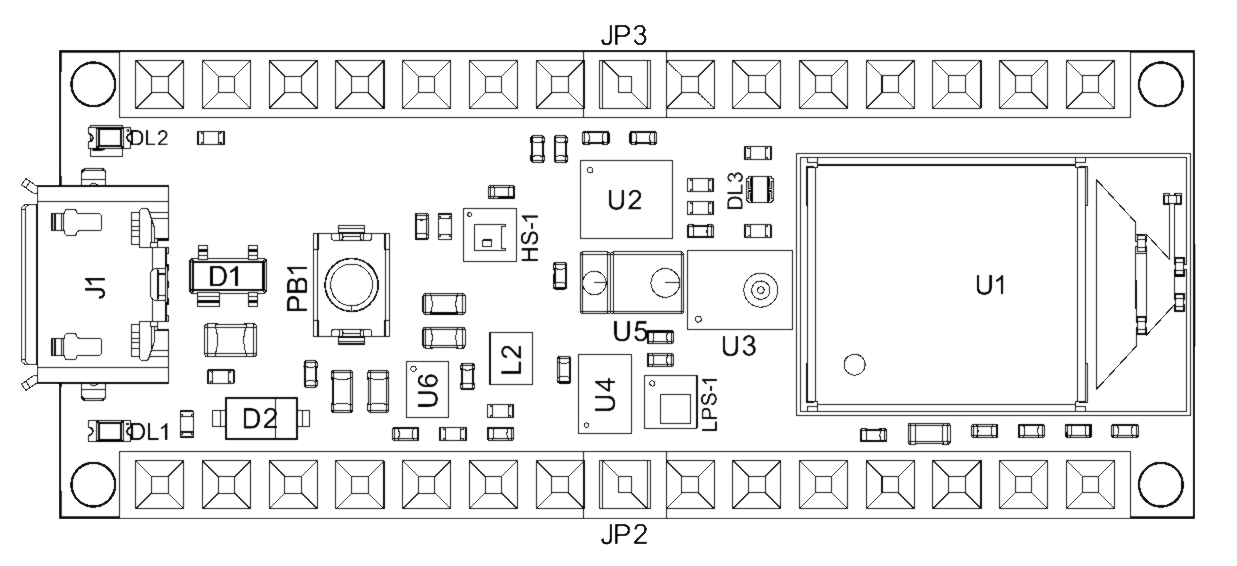
\includegraphics[width=0.8\linewidth]{./ImageFiles/arduino.png}
	\caption{Arduino Nano 33 BLE Sense, vista top. U1: NINA-B306 Module Bluetooth® Low Energy 5.0 Module, U2: LSM9DS1TR Sensor IMU, U3: MP34DT06JTR Mems Microphone, U4: ATECC608A Crypto chip, U5: APDS-9660 Ambient Module, U6: MP2322GQH Step Down Converter, PB1: IT-1185AP1C-160G-GTR Push button, HS-1: HTS221 Humidity Sensor, DL1: Led L, DL2: Led Power.}
	\label{fig:arduino}
\end{figure}
Inoltre, sulla board è presente un chip per la crittografia ATECC608A e un convertitore DC-DC MPM3610. Il microprocessore è integrato nel modulo NINA B306 (\SI{64}{\mega\hertz} Arm Cortex-M4F) che fornisce anche un modulo Bluetooth 5, con supporto multiprotocollo. La board viene alimentata con una tensione di \SI{3.3}{\volt}. Tipicamente, l'alimentazione è fornita tramite la porta USB che viene anche utilizzata per il caricamento del firmware tramite l'Arduino IDE.

Durante il laboratorio è stato testato il funzionamento dell'accelerometro tramite il seguente sketch che permette di ricavare le misure delle accelerazioni proprie dall'accelerometro. Di seguito si riporta il codice del firmware caricato sulla board tramite l'Arudino IDE. In particolare, le misure vengono ricavate dal buffer dell'accelerometro per poi essere scritte sulla porta seriale secondo il formato "{x} {y} {z}".
\lstinputlisting[language=c]{./OtherFiles/firmware.c}

Inoltre, è possibile visualizzare graficamente i dati scritti sulla porta seriale tramite il \textit{Serial Plotter} fornito dall'ambiente di sviluppo di Arduino. Nella figura \ref{fig:serial_plotter} è possibile vedere un esempio di acquisizione dei dati, in cui l'Arduino viene tenuto fermo su un piano. In queste condizioni si noti che l'unica accelerazione misurata è l'accelerazione di gravità con un valore misurato pari a circa \SI{9.9}{\meter \per \second^2}.
\begin{figure}[tbh]
	\centering
	\begin{minipage}{.45\textwidth}
		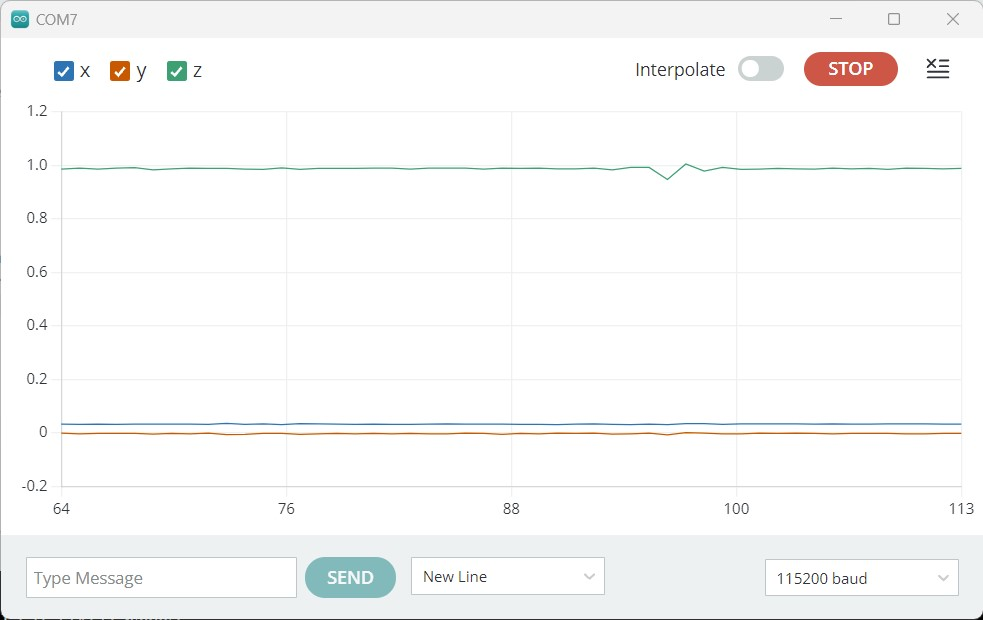
\includegraphics[width=\linewidth]{./ImageFiles/fermo.jpg}
	\end{minipage}
	\begin{minipage}{.45\textwidth}
		\includegraphics[width=\linewidth]{./ImageFiles/testa in giù.jpg}
	\end{minipage}
	\caption{Grafici di alcune misure dell'accelerometro. Nelle immagini si può notare l'accelerazione di gravità misurata sull'asse z con segno positivo (immagine a sinistra) e segno negativo (immagine a destra).}
	\label{fig:serial_plotter}
\end{figure}

Successivamente è stato utilizzato Matlab per analizzare le misure dell'accelerometro ottenute con Arduino. In particolare questi dati sono stati generati muovendo Arduino lungo l'asse x con un tempo di campionamento di \SI{100}{m\second} (in figura \ref{fig:plot_dati}).
\begin{figure}[tbh]
	\centering		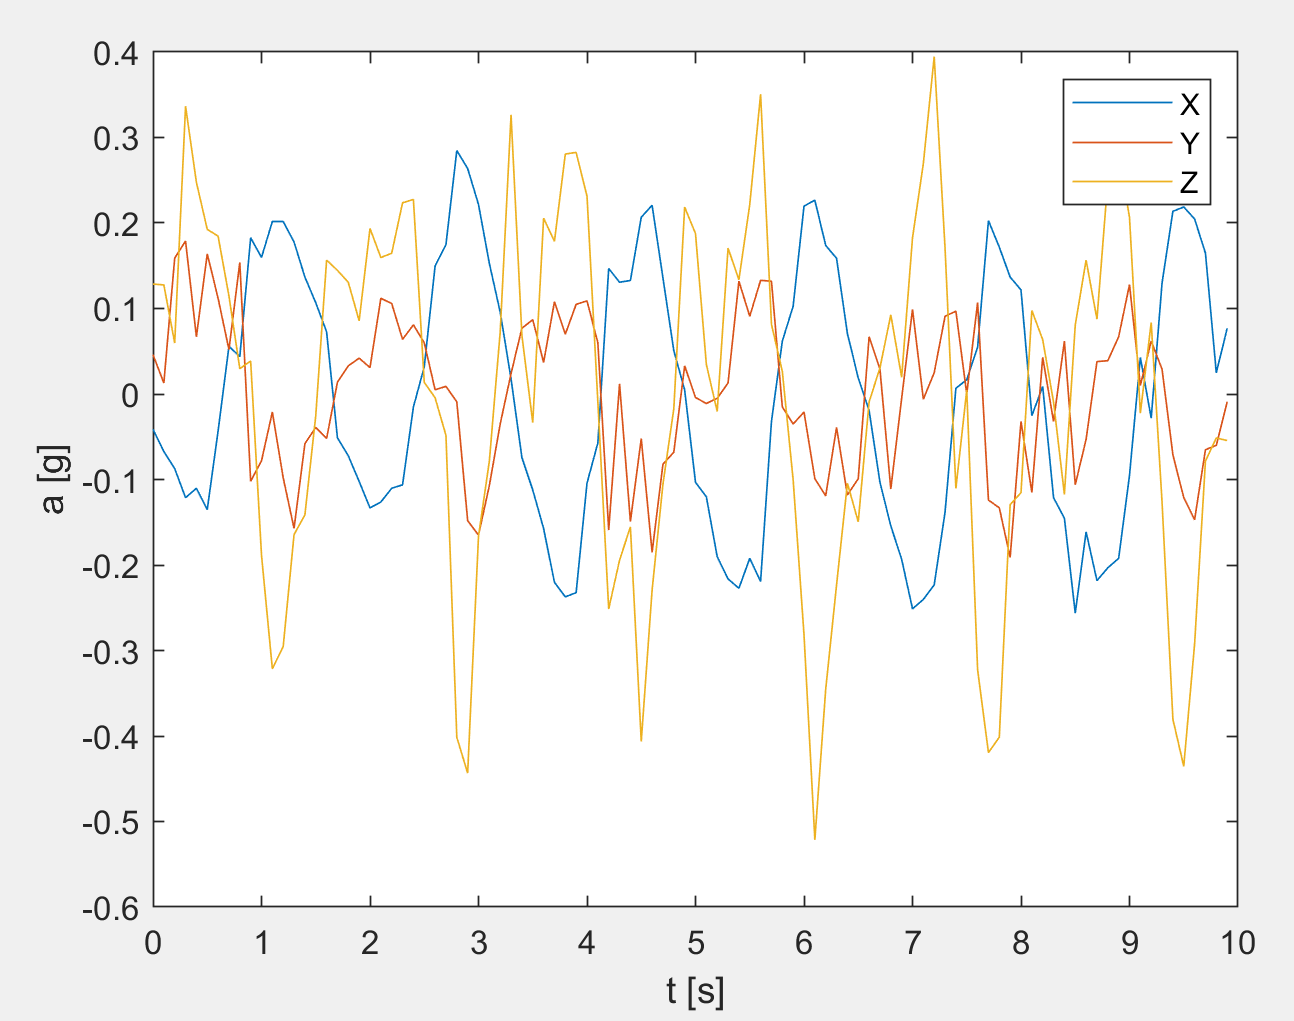
\includegraphics[width=7cm]{./ImageFiles/plot1_arr2.png}
	\caption{Grafico del set di dati grezzi.}
	\label{fig:plot_dati}
\end{figure}

L'obiettivo di questa analisi consiste nell'individuare la frequenza principale del segnale ottenuto dalle misure in seguito a un loro filtraggio realizzato tramite un filtro digitale.

Innanzitutto, per l'implementazione del filtro digitale è stato utilizzato il comando \textit{movmean} di Matlab, che consente di realizzare un filtro digitale a media mobile. In particolare è stato impostato un grado del filtro pari a 10. I dati filtrati sono stati riportati nella figura \ref{fig:plot_dati_filt}.
\begin{figure}[tbh]
	\centering		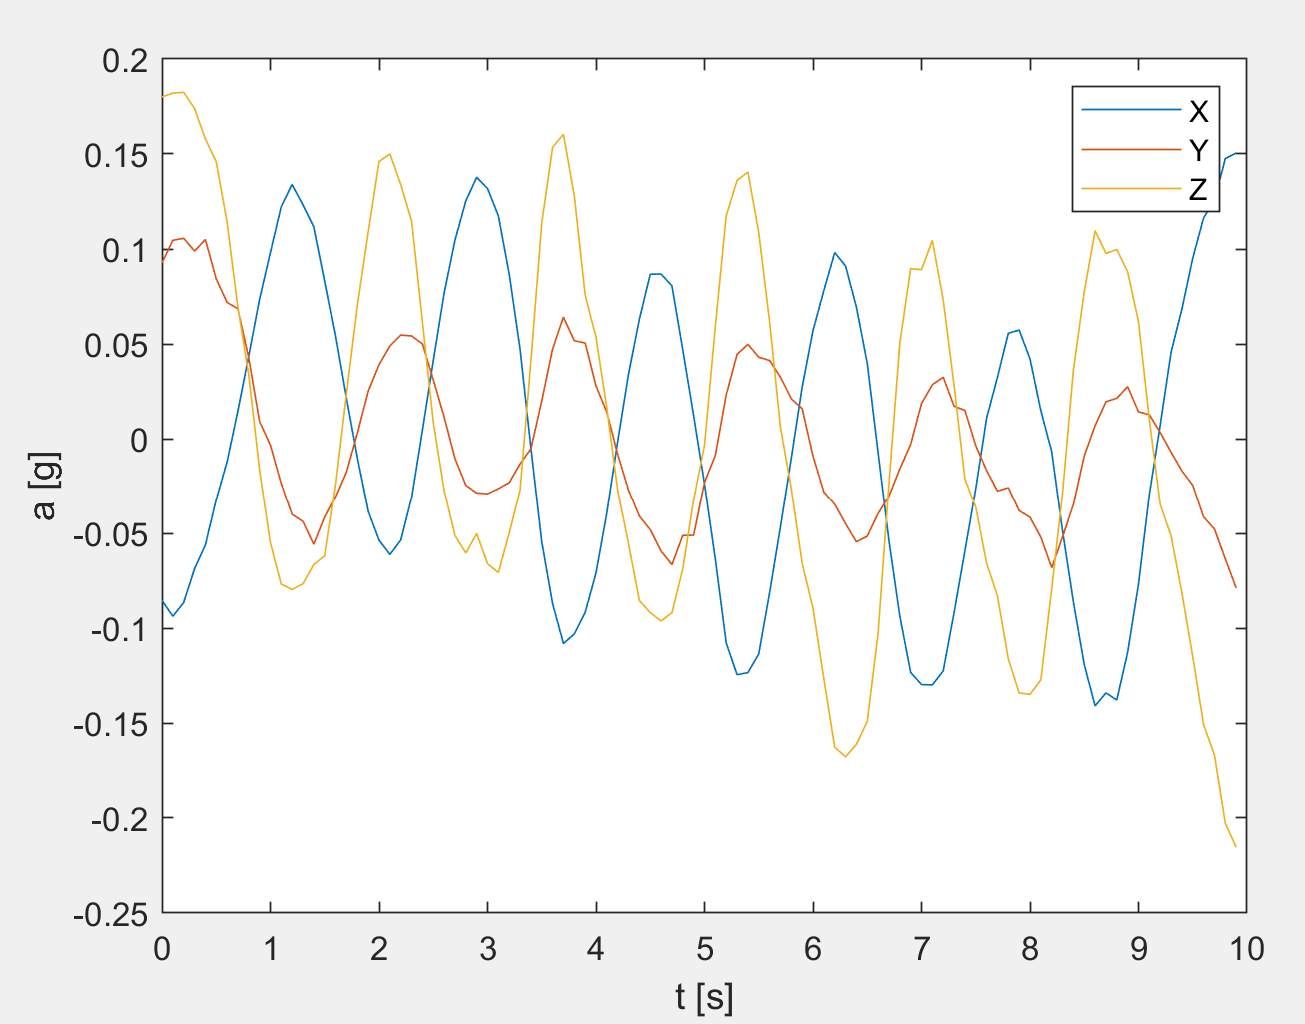
\includegraphics[width=7cm]{./ImageFiles/plot1filt_arr2.png}
	\caption{Grafico del set di dati filtrato.}
	\label{fig:plot_dati_filt}
\end{figure}

In seguito, per determinare il valore della frequenza desiderata sono stati utilizzati due metodi.

Il primo prevede di calcolare i picchi presenti nel segnale: sono stati utilizzati i comandi \textit{gradient} e \textit{diff} di Matlab, che consentono di determinare rispettivamente il gradiente e le differenze tra i gradienti di dati adiacenti e perciò di valutare come la pendenza del segnale filtrato (denominato filt) cambia segno, con lo scopo di rilevare il numero dei picchi presenti nel segnale.
\lstinputlisting[language=Matlab]{./OtherFiles/metodo1.m}

La frequenza risultante dall'applicazione del precedente metodo è pari a \SI{0.6}{\hertz} per ciascuna componente dei dati.

Il secondo metodo, invece, considera la Trasformata di Fourier con il comando \textit{fft} di Matlab ponendo una frequenza di campionamento pari a \SI{10}{\hertz}.
\lstinputlisting[language=Matlab]{./OtherFiles/metodo2.m}

Nella figura \ref{fig:plot_fft} viene messa in evidenza la frequenza principale del segnale filtrato, che risulta essere anche in questo caso pari a \SI{0.6}{\hertz}.
\begin{figure}[tbh]
	\centering		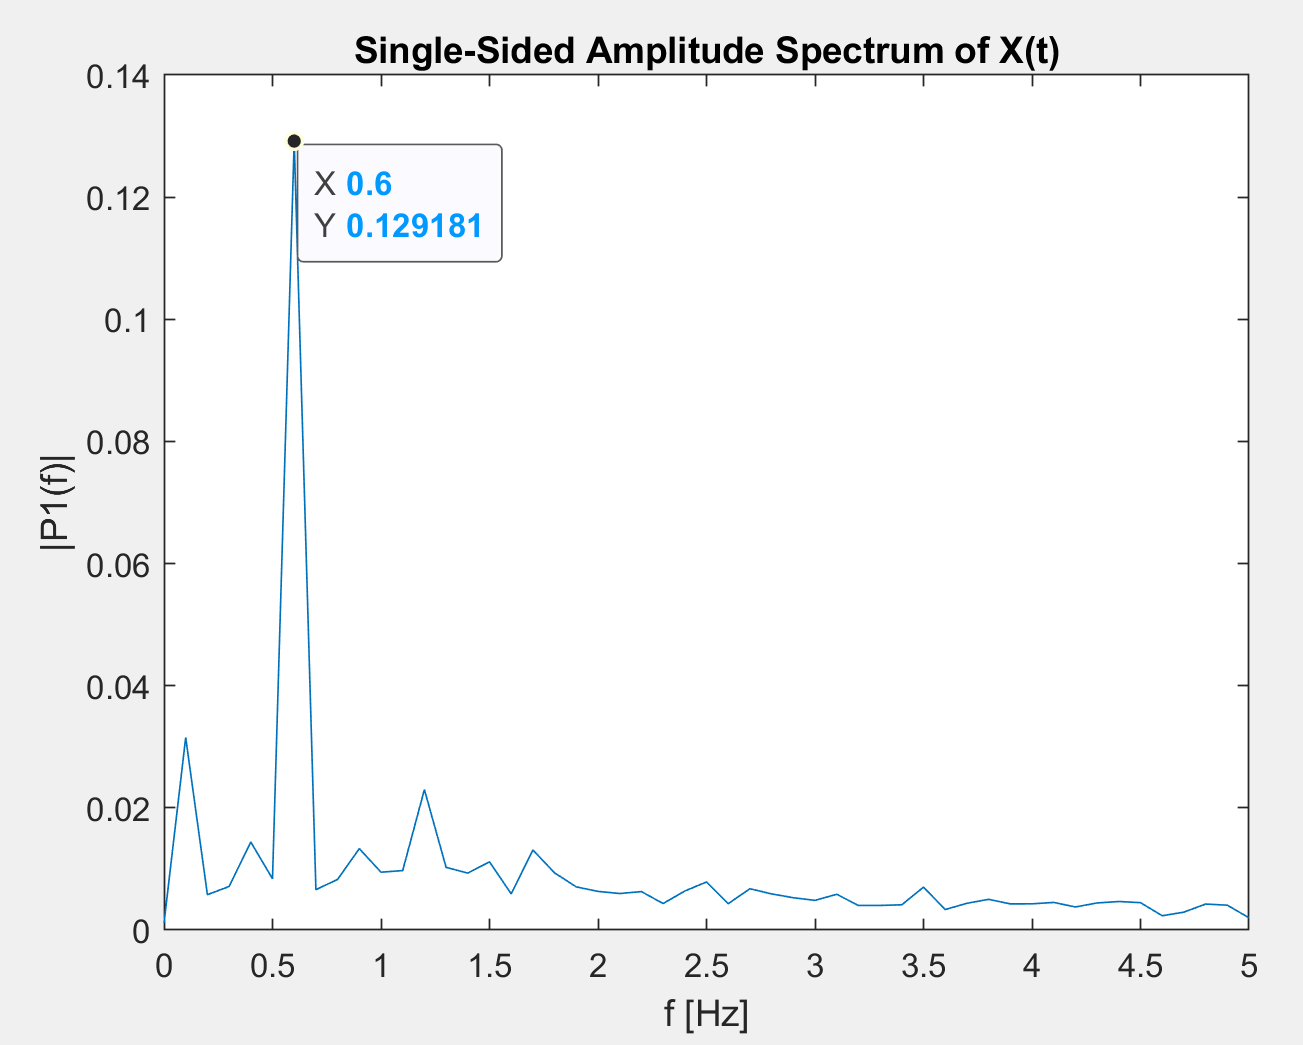
\includegraphics[width=7cm]{./ImageFiles/plot2_arr2.png}
	\caption{Grafico della Trasformata di Fourier del set di dati filtrato.}
	\label{fig:plot_fft}
\end{figure}